\chapter{AFIDs-Pred: Stereotactic Target Localization Using Anatomical Fiducials}\label{chap:afidspred}
\newpage
\sloppy
This chapter is largely based on:
\begin{itemize}[noitemsep,topsep=0pt]
	\item Taha, A., Abbass M., Snyder, M., et al. Optimizing indirect localization of deep brain targets using anatomical fiducials and machine learning. In-Prep.
\end{itemize}

\section{Introduction}

\subsection{Stereotaxy and modern neuroimaging}
The origins of coordinate-based brain mapping can be traced back to Horsley and Clarke \cite{Horsley1908-om}, who designed a stereotaxic apparatus using Cartesian coordinates to localize brain structures relative to cranial landmarks. Building on this foundation, Jean Talairach \cite{Schaltenbrand1977-ge, Talairach1957-eb} leveraged anatomical landmarks, such as the anterior commissure (AC) and posterior commissure (PC), for more refined brain structure localization (i.e., the proportional grid normalization). These early innovations laid the groundwork for population-based brain templates that emerged with the advent of MRI. For example, the MNI305 template \cite{Collins1994-dx} aligned 305 individual MRI scans using AC and PC, overcoming the idiosyncrasies of using a single subject brain as a template. Subsequent advances in non-linear registration further refined these templates, culminating in modern standards such as the MNI152 space \cite{Fonov2009-oi}, now widely employed for aligning anatomical data. Despite these advances, localizing small, poorly visualized structures with millimetric accuracy remains a challenge, particularly when direct anatomical visualization is limited by image resolution, contrast, or artifacts (see Section \ref{sec:SNSX} for a more detailed overview).

\subsection{Millimeters Matter in DBS}
Deep brain stimulation (DBS) is a stereotactic procedure involving the surgical implantation of electrodes in specific brain structures (see Section \ref{sec:whymm} for a more detailed overview). It is well established for the management of a wide array of movement disorders such as Parkinson's disease (PD), essential tremor, dystonia, and Tourette’s syndrome, as well as for select psychiatric conditions including obsessive-compulsive disorder and treatment-resistant depression \cite{Lozano2019-dv}. In the case of movement disorders, small deviations in electrode position during DBS result in side-effects including paresthesias, pyramidal symptoms, diplopia, and dysarthria \cite{Buhmann2017-da}. Meanwhile, sub-optimal placement of the electrode on the order of 2 millimeters (mm) can lead to reduced clinical outcomes \cite{Horn2019-by} and also put patients at risk for post-operative cognitive decline \cite{Reich2022-jf}.

\subsection{Challenges in Localizing DBS Targets}
Achieving the level of precision needed in DBS is complicated by the limitations of clinical neuroimaging. Most MRI scanners used in clinical settings operate at 1.5 or 3 T, which may not always provide the resolution required to clearly visualize small DBS targets such as the STN. Furthermore, patient motion—exacerbated in individuals with movement disorders—suboptimal MRI protocols, and geometric distortions can further degrade image quality \cite{Boutet2021-vg, Chandran2016-eg, Lau2018-fp}. Ultra-high field (UHF; $\geq$7T) MRI enables clear delineation of small brain regions, since increased magnetic field strength yields enhanced signal-to-noise ratio and tissue contrast that can be exploited to improve spatial resolution \cite{Abosch2010-jn, Duchin2012-db, Lau2017-ea, Lau2020-dh, Lenglet2012-ii}. However, UHF-MRI systems are not commonly available, limiting widespread clinical adoption \cite{Clarke2020-ky}. As a result, DBS targeting may employ indirect localization techniques that rely on predefined coordinate spaces.

\subsection{Indirect Brain Target Localization Approaches}
Existing methods for indirect localization can be grouped into two categories: (1) atlas-based consensus coordinates and (2) atlas-based registration. Atlas-based coordinate approaches describe consensus coordinates of a target relative to the midpoint along the AC-PC line, known as the mid-commissural point (MCP). The MCP is susceptible to intersubject variability, as no single atlas-based consensus coordinate perfectly captures the anatomical differences observed across populations. Meanwhile, atlas-based (i.e., deformable) registration techniques estimate the deformation field used to propagate atlas labels from a stereotactic space (e.g., MNI) to individual brains. Deformable registration yields errors on the order of 1-5 mm \cite{Lau2019-eh, Abbass2022-lf, Miller2023-ct}, with lower quality clinical scans prone to failing thus requiring manual intervention. Furthermore, surgical planning often occurs on gadolinium enhanced T1w scans (MRI-gad), to ensure safe implantation of electrodes while avoiding blood vessels, introducing further complexity to the  registration process \cite{Abbass2022-lf, Abbass2025-el} and application of standard neuroimaging workflows which may not be optimized for MRI-gad \cite{Ogunsanya2024-uf, Warntjes2014-wy}.

\subsection{Machine Learning for Automatic Brain Target Localization}
Machine learning (ML) models for automatic localization of brain structures have gained significant interest offering a faster and more generalizable alternative to deformable registration \cite{Baniasadi2023-lm, Ren2025-zu}. However, only a limited number of studies evaluated and adapted ML frameworks to the small DBS targets while achieving generalizability on clinical quality (e.g., MRI-gad) scans \cite{Baniasadi2023-lm}. Furthermore, due to the intensive process of acquiring manual ground-truth labels, many approaches have focused on matching accuracy of well-curated parameters during deformable registration approaches (i.e., training labels generated from quality controlled deformable registration segmentation data) \cite{Baniasadi2023-lm}.


\subsection{Coordinate-to-Coordinate Machine Learning Framework}
In this study, we validate an ML framework to accurately localize brain structures solely from $x$, $y$, $z$ coordinates of surrounding anatomical landmarks (i.e., coordinate-to-coordinate). Our target localization approach is dependent only on validated anatomical landmarks inspired from classical stereotactic methods \cite{Lau2019-eh, Abbass2022-lf}, which are reproducible across various MRI field strengths and modalities (see Chapter \ref{chap:afidsdata}). This framework was designed with generalizability and explainability in mind, such that it can be applied to other brain targets while enabling understanding of relationships between predefined landmarks and the targeted brain region, including structures targeted in DBS (i.e., STN). Our framework integrates well within the clinical workflow, which already involves preoperative localization of landmarks (e.g., AC and PC). Central to our approach is an open-source framework, which involves the release of our coordinate data, code, and our framework in the form of a website \url{www.stereotaxy.afids.io}.

\begin{figure}[hbt!]
    \centering
    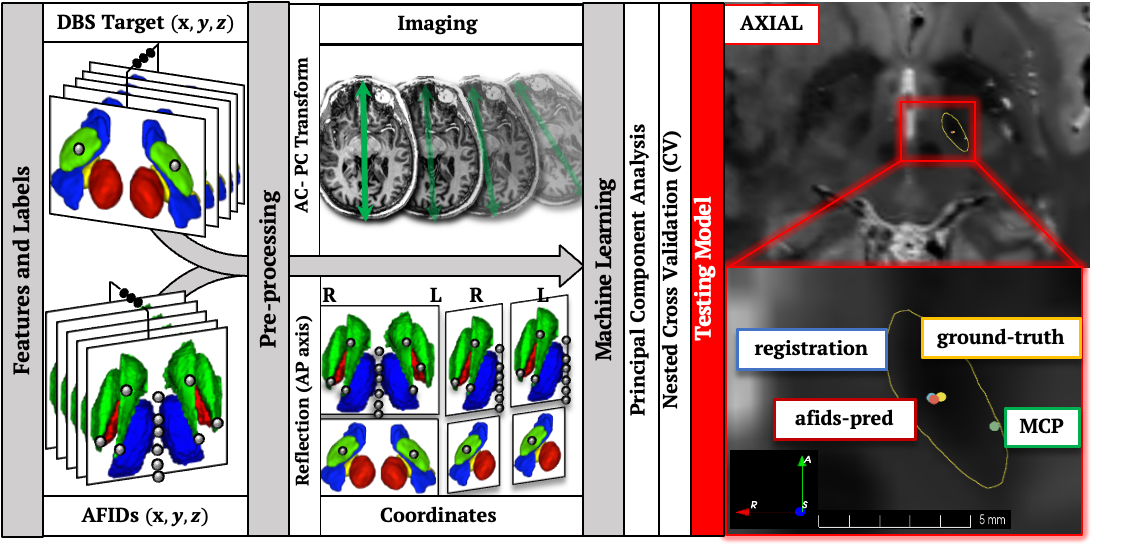
\includegraphics[width=1\linewidth]{figs/ch4_Figure_afidspred.png}
    \caption{Overall workflow for building our machine learning model to localize the subthalamic nucleus (STN) using anatomical fiducials (AFIDs). Validated AFID coordinates were used as features to predict STN coordinates. All coordinates were anterior commissure (AC) and posterior commissure (PC) aligned. AFID and STN coordinates on the right hemisphere were mirrored to augment data. Principal component analysis (PCA) was performed on coordinate data to capture collinearity. A nested 4-fold cross validation strategy was employed to train a linear machine learning model. Model prediction was validated on various imaging modalities and compared to deformable registration for STN localization.}
    \label{fig:ch4_Figure_afidspred}
\end{figure}

\section{Methods}

\subsection{Participants}
We leverage 202 MRI scans on which we have more than 6,500 ground truth anatomical landmarks applied in accordance with a validated annotation protocol \cite{Lau2019-eh} by more than 20 human raters (Table \ref{tab:afidpred_datasets}). Although this dataset has been described in previously in Chapter \ref{chap:afidsdata}, we provide below details to datasets of the dataset as it pretains to this chapter: 

\texttt{The Stereotactic Neurosurgery (SNSX) dataset.} This dataset consists of 61 participants (32 healthy controls and 30 scheduled for DBS). Participants were imaged using a 7T head-only MRI scanner (Siemens Magnetom; Siemens Healthineers, Erlangen, Germany) at the Center for Functional and Metabolic Mapping (CFMM) in Western University (REB: 109045). The MRI sequences used for this study were: 1) 3D T1w MP2RAGE  and 2) 3D optimized T2w fast-spin echo (T2 SPACE).

\texttt{The London Health Sciences Center Parkinson’s Disease (LHSCPD) dataset.} This dataset consists of a subset (n = 10) of the same participants as in the SNSX dataset, scheduled to undergo DBS at London Health Sciences Center (LHSC; REB: R-17-156). Participants were imaged using a 1.5T MRI scanner (Signa, 1.5T, General Electric, Milwaukee, Wisconsin, USA). The MRI sequence used in this study was a 3D T1w MP2RAGE with gadolinium contrast (termed “MRI-gad” in subsequent sections).

\texttt{An openly released 3T and 7T (3T-7T) dataset} \cite{Chen2023-cn}, consisting of healthy participants (n = 10) imaged using the following sequences: 1) 3D T1w MP2RAGE and 2) 3D T2 SPACE. Participants are imaged at both 3T and 7T (i.e., test-retest).

\texttt{A subset of a previously released (afids-data) dataset}, which aggregated brain landmark annotations (n = 110) on various populations (healthy, abnormal ventricular size, and PD). This dataset is independent of the previously mentioned datasets.

\begin{table}[h!]
\centering
\caption{Various datasets leveraged as part of this study, all of which have curated anatomical landmark annotations.}
\begin{tabularx}{\textwidth}{l l l l l}
\toprule
\textbf{Dataset} & \textbf{Field Strength (T)} & \textbf{Disease (n)} & \textbf{Analysis} \\
\midrule
SNSX* & 7 & HC (32), PD (30) & Training and Testing  \\
LHSCPD & 1.5 (paired SNSX) & PD (10) & Clinical Validation \\
3T-7T* & 3 and 7 (paired) & HC (10) & External Validation  \\
afids-data & 1.5, 3, and 7 & HC (60), PD (40), AD (10) & Landmark Generalization \\
Template & 3 & HC (1) & Landmark Augmentation  \\
\bottomrule
\end{tabularx}

\vspace{1ex}
\raggedright
\footnotesize{
\textbf{HC} = healthy control, \textbf{PD} = Parkinson’s disease, \textbf{AD} = Alzheimer’s disease.\\
* Contains manual human rater curated subthalamic nucleus (STN) segmentations.
}
\label{tab:afidpred_datasets}
\end{table}

\subsection{Coordinate Data Annotation}
We employ a previously validated protocol for the annotation of anatomical fiducials (AFIDs; \url{https://afids.github.io/afids-protocol}) providing a point-based sampling of multiple brain structures. In this study, we selected a subset of 16 AFIDs (see Supplementary Figure S1) described by the protocol which (1) circumscribe the midbrain and surrounding structures (e.g., DBS targets) and (2) can be localized within 1 mm by expert and novice human raters.

\textbf{AFID Annotations:} All annotations were performed in accordance with the AFIDs protocol via 3DSlicer 4.10. Rater placements per AFID were averaged to curate the ground-truth coordinates (x, y, and z).

\textbf{STN Annotations:} All annotations were performed via 3DSlicer 4.10 \cite{ref} using the smallest configuration of the paint brush (1 mm) and the pencil drawing tool on 7T T2w imaging. Rater segmentations per subject were selected via majority voting (>50\%) and then collapsed to a center of mass representing the STN centroid, constituting the ground truth STN centroid coordinates (x, y, z).

Each scan was annotated by at least two human raters (see Supplementary Table S1 for a breakdown of rater demographic data). The ground truth coordinates were quality controlled (QC) by three raters (AT, JZ, and EC). We provide example QC files (*.html format; see Supplementary Attachment A) with accompanying code and ground truth coordinates (*.fcsv) used in this work \cite{ref}. Supplementary Attachment B provides a full 3D-visualization of the coordinates across all datasets.

\subsection{Coordinate Data Processing}
An AC-PC alignment was performed followed by centering coordinates at the mid-commissural point (MCP; defined as the midpoint between AC and PC). Coordinates on the left hemisphere were reflected to the right by inverting the sign of the x-coordinate after AC-PC transformation and MCP centering. Thus, each participant constituted two augmented examples. Preliminary analysis using training data was conducted to investigate correlations across coordinates to inform ML. Subsequently, principal component analysis (PCA) was performed on concatenated x, y, z coordinates. Top principal components (PCs) capturing 99\% of the variance were retained for subsequent ML model training.

\subsection{Data Split and Machine Learning}
AFID and STN coordinate data of participants from the SNSX dataset were used for ML training. Ten participants from the SNSX dataset were assigned to a reserved testing dataset used solely to report the accuracy of our model. These participants were also the same ones from the LHSCPD dataset, enabling evaluation of our model on clinical quality 1.5T MRI-gad scans. Finally, the 3T-7T dataset was used for external validation to report prediction accuracy at 3T and 7T MRI.

To explore the trade-off between model simplicity and complexity, we evaluated two ML algorithms: (1) Ridge Regression \cite{ref}, a linear model with built-in regularization, and (2) Extreme Gradient Boosting (XGBoost) \cite{ref}, a more complex ensemble-based method capable of modeling non-linear relationships.

ML models were trained via a nested cross-validation (CV) strategy to tune hyperparameters and evaluate performance (scikit-learn; \cite{pedregosa2012}). The outer CV loop involved a 4-fold split of all training data for statistically evaluating the two ML models, and the inner CV loop involved a 3-fold split CV strategy for tuning hyperparameters. All the folds were curated such that for a given training example (i.e., participant), the left and right hemisphere target labels (e.g., STN) were grouped together. This prevented a scenario where the left and right labels appear separately across training and testing, protecting against over-reporting accuracy or data leakage due to hemispheric symmetry. Furthermore, group-based preprocessing (i.e., PCA) was performed independently within each fold to prevent leakage across folds. Final model accuracy was reported on the four testing sets curated by the outer CV loops. We compute the x, y, z mean squared error (MSE) and Euclidean distance (ED) to evaluate models. See Figure~\ref{fig:workflow} for an end-to-end abstraction of our methodology.

\subsection{Model Robustness, Generalizability, and Comparative Evaluation}

\textbf{Generalization to Other Imaging Modalities:} To investigate model precision on clinical quality imaging, model coordinate predictions on 1.5T MRI-gad scans were statistically compared to 7T counterpart MRI scans in AC-PC space. This paired coordinate-based statistical analysis was leveraged to investigate model precision, as curating ground-truth STN annotations was not feasible on clinical imaging. To further demonstrate robustness, we leveraged AFID and STN annotations on an external 3T-7T paired dataset. A similar analysis was conducted using 7T T2w MRI as ground truth.

\textbf{Benchmarking:} We performed statistical comparisons between our model and deformable registration for STN localization using our 1.5T MRI-gad dataset (i.e., LHSCPD) and paired 7T-MRI counterpart (i.e., SNSXPD). The Distal atlas segmentations in MNI space \cite{chakravarty2006, ewert2018} were warped to native space using presets from a nonlinear deformation framework validated via 11,000 non-linear warps across more than 100 subjects \cite{ewert2019}. We apply this framework as implemented in Lead-DBS software \cite{ref}. All methods were analyzed using a signed-Wilcoxon Rank Test. Bonferroni multiple comparison correction was applied where necessary.

\textbf{Robustness to Annotation Variability:} To investigate model dependency on accurate localization, we used 38 independent AFID protocol applications in a common space (i.e., MNI) and evaluated STN prediction accuracy across these trials. For this analysis, the AFID protocol was applied independently by 10 human raters with varying neuroanatomical expertise.

\textbf{Landmark Prediction Generalizability:} To investigate the generalizability of our framework to other brain landmarks, we iteratively dropped each AFID (i.e., leave-one-AFID out) and predicted it using the other AFIDs. This analysis was conducted using all datasets (i.e., n = 202) and employed the same nested cross-validation approach described in Section~2.4.

\subsection{Model Deployment}
Building on the previous open software infrastructure of the AFID project, we deploy our model on an online web app (\url{https://afids-stereotaxy-predict.onrender.com}). This enables users to upload their AFID placements as specified by our modified protocol (See Supplementary Attachment C) and receive STN coordinate predictions alongside a 3DSlicer-compatible AC-PC transformation matrix.


\section{Results}

\subsection{Rater Curated Data}
Demographic data for human raters involved in annotations are made available in Supplementary Table~S1. The localization error across all AFID placements and datasets was 0.84~$\pm$~0.31~mm. The inter-rater STN segmentation overlap was 0.78~$\pm$~0.03, measured using the Dice similarity coefficient. There was no statistical difference between right and left hemisphere STN segmentations, thus they were combined in subsequent descriptive summaries.

The average volumes of the STN for the healthy control (HC) and Parkinson’s disease (PD) cohorts were 136.56~$\pm$~16.24~mm\textsuperscript{3} and 128.03~$\pm$~29.67~mm\textsuperscript{3}, respectively ($p = 0.047$; Mann–Whitney U test). The average x, y, z STN coordinates in MCP space for the HC and PD cohorts were: 10.18, -0.92, -3.27 and 10.14, -0.88, -3.61, respectively (x: $p = 0.93$, y: $p = 0.91$, z: $p = 0.002$; Mann–Whitney U test). Only the z-coordinate was statistically significant after Bonferroni correction ($\alpha = 0.05/4$).

\subsection{Preliminary Analysis and Principal Component Analysis (PCA)}
The x, y, z coordinates of AFIDs from all datasets excluding testing data were correlated with each other, revealing a strong linear correlation (see Figure~\ref{fig:pca_corr}). This finding motivated using PCA to reduce the number of features used for ML model training. The top 36 principal components (PCs) captured 99\% of the variation in the data (see Figure~\ref{fig:pca_variance}) and were chosen for subsequent analysis. Further exploration of AFID contributions to PCs revealed relatively broad distribution (see Figure~\ref{fig:pca_loadings}). Coordinates of AFIDs using training data were plotted with STN x, y, z coordinates, revealing strong linear correlations (see Figure~\ref{fig:pca_stn_corr}), motivating the use of a linear regression ML model.

\subsection{Machine Learning Model Performance}
\textbf{Model Training:} A multi-output paradigm using nested CV was used to train a Ridge Regressor and an XGBRegressor. Euclidean Distance (ED) computed on the outer CV folds was compared using a Wilcoxon signed-rank test, and the Ridge Regressor statistically outperformed the XGBRegressor ($\alpha = 0.05$, $p < 0.01$), supporting its use for predicting STN coordinates.

\textbf{Model Testing:} The average x, y, z mean squared errors (MSE) across all testing data (40 STNs) were: 0.45~$\pm$~0.56~mm, 0.66~$\pm$~0.79~mm, and 0.48~$\pm$~0.58~mm, respectively. The overall median ED error was 1.20~$\pm$~0.44~mm (IQR: 0.84–1.52). See Table~\ref{table:ml_results} for a more granular breakdown of results.

\subsection{Model Generalizability and Comparisons}

\textbf{Validation across Other Imaging Modalities:} We evaluated model performance across different imaging modalities by analyzing paired datasets acquired at various field strengths (see Figure~\ref{fig:paired_modalities}). Ten participants with both 1.5T MRI-gad (LHSCPD) and 7T MRI-nogad (SNSX), as well as ten participants with both 3T and 7T MRI (3T-7T), were included (see Section~2.4). Wilcoxon signed-rank test with Bonferroni correction ($\alpha = 0.05/4$) revealed no significant differences in x, y, z MSE and ED across the two paired imaging modalities.

\textbf{Model Comparison and Performance Benchmarking:} We benchmarked our model against deformable registration (see Figure~\ref{fig:benchmarking}). On 1.5T MRI-gad scans, our model statistically outperformed registration ($p < 0.001$). Conversely, on multispectral 7T MRI-nogad data (i.e., registration warps computed using both T1 and T2 imaging), no significant difference in performance was observed between registration and our model ($p > 0.1$).

\textbf{Feature Importance and Augmentation:} To assess the influence of landmark annotation error on model performance, we examined the relationship between rater localization error and prediction error. A moderate correlation was observed (Pearson $r = 0.47$; $p < 0.01$), with regression analysis revealing a slope of 0.46 (see Figure~\ref{fig:importance}).

\textbf{Generalizability to Other Brain Landmarks:} To assess the broader applicability of our framework, we extended the localization approach to nine additional midbrain landmarks (see Figure~\ref{fig:generalization}). The model maintained high accuracy across these structures, achieving a median ED of 1.27~$\pm$~0.96~mm (IQR: 0.73–2.00).

\subsection{Clinical Use Cases}
We tested the functionality of our web-app by employing it in two DBS cases at our center.

\textbf{Case 1:} Our framework was independently applied on multimodal data (see Figure~\ref{fig:case1}). Predictions were within 1~mm when using any of the following modalities: (1) 1.5T MRI-gad, 7T T1w-MRI, 7T T2w-MRI, and CT with Contrast.

\textbf{Case 2:} Our model was applied on post-operative MRI scans from a DBS electrode re-implantation case (see Figure~\ref{fig:case2}).

